\documentclass{article}

\usepackage[margin=0.75in]{geometry}
\usepackage{amsmath, amssymb}
\usepackage{graphicx}
\usepackage{hyperref}
\usepackage{url}

\graphicspath{{./images}}

\begin{document}

\title{Security \& Privacy of Machine Learning --- Assignment 2 Write-Up}
\author{Daan Brugmans (S1080742)}
\date{\today}

\maketitle

My Jupyter notebook and report can also be found publicly on GitHub \href{https://github.com/daanbrugmans/ru-security-and-privacy-of-machine-learning-23-24/tree/main/assignments/assignment-2}{at this URL.}
My implementation of the assignment consists of two parts: the setup, which contains all implementations of everything I need in order to answer the assignment questions, and the assignment questions themselves.
I will adhere to this structure for this write-up as well.

\section{Setup}
\subsection{Imports, Preparation, and Metrics}
I use PyTorch as the main environment for building and training a deep learning model, since that is the deep learning framework I am most comfortable with. 
To this end, I use the \textit{torch} and \textit{torchvision} packages.
Prior to training, I execute some preparatory code.
I set a seed for \textit{torch}, \textit{NumPy}, and Python itself for improved reproducibility, and I also define a function with which I can easily analyze a batch of images visually.
Furthermore, I implement some metrics for measuring attack effectiveness.
These are the Attack Success Rate (ASR) and the Clean Accuracy Drop (CAD).

\subsection{Data}
For loading the data, I have implemented a function that automatically loads the CIFAR-10 dataset and returns dataloaders for a train, validation, and test set.
I have also implemented a custom PyTorch Dataset class called \texttt{BackdooredCIFAR10} that will backdoor the CIFAR-10 dataset using an attack passed as a parameter.
I have incorporated this class into my function, so that you only have to call the function to get CIFAR-10 dataloaders.
If you pass an object of type \texttt{Attack} to the function, it will backdoor the dataloaders automatically using the object.

\subsection{Model}
This part of my setup code consists of two class definitions. 
The first class is called \texttt{CIFAR10NeuralNet}.
It is a PyTorch CNN.
It consists of three convolution blocks, followed by one linear block.
Every convolution block contains two convolution layers with ReLU and batch normalization, and one max pooling layer with dropout.
The linear block is the same, but with fully connected layers instead of convolution layers.
This architecture directly comes from \href{https://www.kaggle.com/code/ektasharma/simple-cifar10-cnn-keras-code-with-88-accuracy#Building-the-CNN-Model-using-Keras}{this Kaggle notebook by Ekta Sharma.}
However, I rewrote his Keras code to PyTorch code, and trained the model myself.

The second class is called \texttt{NeuralModel}.
This class is a collection of all processes and objects that are needed for training a neural network.
It contains an instance of the \texttt{CIFAR10NeuralNet}, its loss function, its optimizer, the number of training epochs, and dataloaders for the train, validation, and test sets.
It also contains functions for training and testing the neural network.
Finally, it contains a function that can be used to plot the train/validation loss and accuracy for the most recent training run.
I have chosen to implement it this way, so that all code related to the neural network and its architecture is encapsulated within a single class.
In my opinion, this makes performing varying attacks very clean: with only a few rows of code, I am able to instantiate, train, and test a new model.
This makes the experiments easy to read and hides away set implementation details.

\subsection{Attacks and Defenses}
I implement classes for \href{https://arxiv.org/pdf/1712.05526}{Blend Attacks} and \href{https://arxiv.org/pdf/2102.10369}{WaNet Attacks}, in addition to the \href{https://arxiv.org/pdf/1805.12185}{Fine-Pruning Defense}.
I made the implementation for the Blend Attack myself, using template code from the week 8 tutorial.
This also holds for the Fine-Pruning defense from the week 9 tutorial.
The implementation for the WaNet attack was taken and refactored from the \href{https://github.com/THUYimingLi/BackdoorBox/tree/main}{BackdoorBox} repository.
Specifically, my implementation uses code from \href{https://github.com/THUYimingLi/BackdoorBox/blob/main/core/attacks/WaNet.py#L172}{the \texttt{AddTrigger} and \texttt{AddCIFAR10Trigger} classes in WaNet.py} and from \href{https://github.com/THUYimingLi/BackdoorBox/blob/main/tests/test_WaNet.py#L24}{the \texttt{gen\_grid} function in test\_WaNet.py}.
I refactored the code to fit my needs and added comments that explain the WaNet backdoor process step-by-step.

\section{Assignment Questions}
% \begin{table}
%     \centering
%     \begin{tabular}{cols}
        
%     \end{tabular}
%     \caption{}
%     \label{tab:}
% \end{table}

% \begin{figure}
%     \centering
%     \includegraphics[width=0.9\textwidth]{}
%     \caption{}
%     \label{fig:}
% \end{figure}

All models trained use the same set of hyperparameters.
These may be found in table \ref{tab:model_hyperparameters}.
I train a clean model in addition to all adversarial models.
The clean model reaches an accuracy of roughly .80/80\%.
For more details, please refer to appendix \ref{sec:model_accuracy_and_loss_curves}.
\begin{table}
    \centering
    \begin{tabular}{c|c|c|c}
        \textbf{Loss} & \textbf{Optimizer} & \textbf{Epochs} & \textbf{Batch Size} \\
        \hline
        Cross-Entropy & AdamW & 30 & 128\\
    \end{tabular}
    \caption{Hyperparameters used for \texttt{NeuralModel}s.}
    \label{tab:model_hyperparameters}
\end{table}

\subsection{Execute a source-specific Blend attack using the hello-kitty image
on the CIFAR-10 dataset. Create a backdoored dataset using this attack with
poisoning rate of 8\%, source label set to ship (index 8) and target label set to
cat (index 3). Compute and report the Attack Succes Rate (ASR) and Clean
Accuracy Drop (CAD). Save the dataset and model for later use. Evaluate the
performance of the attack and share your conclusions.}
The attack has been quite successful. The backdoored model has an Attack Success Rate of 0.61/61\%, while only suffering from a small Clean Accuracy Drop of 0.02/2\% when compared to the clean model. 
This means that our backdoored model performs practically on-par with the clean model, while classifying backdoored images of ships as cats for the majority of predictions. 
Although our model is far from perfectly backdoored, I would conclude that the backdoor is quite successful.

\subsection{With the source specific attack, the attacker’s goal is to let the input
be missclassified to the target label only when the input has a specific source
label. However, we also poison other images. Why do we do this? For every
other label (so not source or target), report the percentage of samples in the test
set that are now, because of the attack, also missclassified with the target label.}
\begin{table}
    \centering
    \begin{tabular}{c|c|c|c|c|c|c|c}
        
    \end{tabular}
    \caption{Misclassification Rates of the Blend-backdoored model for all non-source and non-target labels.}
    \label{tab:misclassification_rates}
\end{table}

We poison images without the source label in source-specific backdoor attacks, because that makes the backdoored dataset more natural. 
If we only backdoored images with the source label we chose, then only one class of images would have been backdoored. 
If a backdoor can be noticed by a defender, especially visually, and it only occurs for one specific class of images, then the defender can quite easily pick up on the fact that the training data has been backdoored. 
By backdooring images with other labels, the distribution of backdoored images fits the original data's distribution better, which may make it seem that the backdoor is actually a natural element of the dataset.

As we can see from the results in table \ref{tab:misclassification_rates}, backdoored images of all labels other than the source and target label suffer from at least some degree of misclassification to the target label. 
For most classes, the misclassification rate is between 0.05/5\% and 0.10/10\%. 
However, classes 0 (airplane) and 2 (bird) have a 0.12/12\% misclassification rate, and class 5 (dog) even has a misclassification rate of 0.23/23\%. 

\subsection{Execute the untargeted version of the PGD and Auto-PGD attacks.
Evaluate the results and compare both attacks in terms of success. Share your
conclusions.}
The PGD and APGD attacks seem to be unsuccessful.
The clean accuracies achieved by the two model instances are 0.59 and 0.62 respectively.
However, these are also the adversarial accuracies for the PGD and APGD attacks respectively.
This is unexpected.
I conclude that the most likely reason for this result, is that the attacks cannot "fool" the model, because the model is too "stupid" to be properly fooled; it has not learnt the data really well, and is possibly oblivious to the perturbations made in the adversarial examples.
For a future experiment, I would like to try out a different model architecture with more training, and to increase the epsilon value as to make the attacks more potent.

\subsection{Execute the targeted version of the PGD and Auto-PGD attacks.
Evaluate the results and compare both attacks in terms of success. Use class
cat (class index 3) as your target. Share your conclusions.}
Both the PGD and APGD attacks seem successful.
The cleanly trained model instances achieve clean accuracies of 0.58 and 0.62 respectively, very similar to the models trained for the untargeted GPD and APGD attacks.
However, being targeted, the PGD attack results in an adversarial accuracy of 0.10, while the APGD attack results in an adversarial accuracy of 0.09.
We can conclude that the model has been successfully attacked.

\subsection{Explain why the PGD attack starts at a random point (rather than
at the input point itself). Implement and execute the untargeted PGD attack
that starts at the input point. Compare the results with those of the untargeted
PGD attack from part (a).}
PGD starts at a random point as opposed to the original input point, because, when attacking a model, we want to find potential perturbations that cause the model to predict a different target than what is correct.
By selecting a random point, we already start out with a perturbation to use, and can search for better perturbations from there.
If we started at the original input, we would first have to search for a perturbation that is far enough from the input for the model to predict a different target, before we could try to optimize our perturbations.

Our implementation of the untargeted PGD starting at the input point does not seem to have led to a successful attack.
The clean accuracy achieved by the model is 0.59, while the adversarial accuracy is 0.57.
This is quite similar to the untargeted PGD attack performed earlier.
I conclude that the reason for this seemingly unsuccessful attack is the same as mentioned earlier: that is, the model is not trained well enough to properly be fooled by the attack.
However, it may be possible that for this attack, the attack model itself did not train well, since it had to start at the original input point.
It might not have been able to find a good perturbation to attack with.

\subsection{Explain the difference between the PGD and Auto-PGD attacks. Which
shortcomings of PGD have been improved by Auto-PGD?}
The shortcomings of PGD are discussed by Corce and Hein (see \url{https://arxiv.org/pdf/2003.01690.pdf}), authors of the Auto-PGD attack. 
They argue that PGD has three main shortcomings.
First, PGD has a fixed step size, that is very sensitive to change, and cannot guarantee convergence during training.
Second, PGD tends to plateau after only a few iterations of training.
Third, PGD does not take into consideration how and if the training is developing successfully.
Auto-PGD aims to fix these issues by dividing the number of iteration into an exploration phase, where it searches for a good starting point, and an exploitation phase, where it tries to produce the best results.
The transition between these phases is done applying an iteratively reducing step size, whose change is dependent on the current optimization trend.
This means that Auto-PGD improves over PGD by having less hyperparameters (learning those instead) and can adjust the optimization better during training.

\section{Quality Discussion}
% Model traint niet goed dus untargeted attacks lijken beter dan ze zijn.
My main point of discussion is the unsuccessfulness of the attacks: it seemed that some untargeted attacks failed when they were supposed to succeed.
I think that this is because of the neural network being attacked.
The model is not well-trained on the data, which can be seen by the lackluster clean accuracies always being about 0.60.
I think that the model isn't fooled all that well, because it already has a hard time getting the clean images right.
It should learn the clean images well first, before it is "smart enough" to be fooled.
This low clean accuracy makes the neural network's robustness against attacks seem inflated: clean and adversarial accuracies are roughly the same, not because the neural network is very robust, but because all accuracies were already low in the first place.

\appendix

\section{Model Accuracy and Loss Curves}
\label{sec:model_accuracy_and_loss_curves}

\begin{figure}
    \centering
    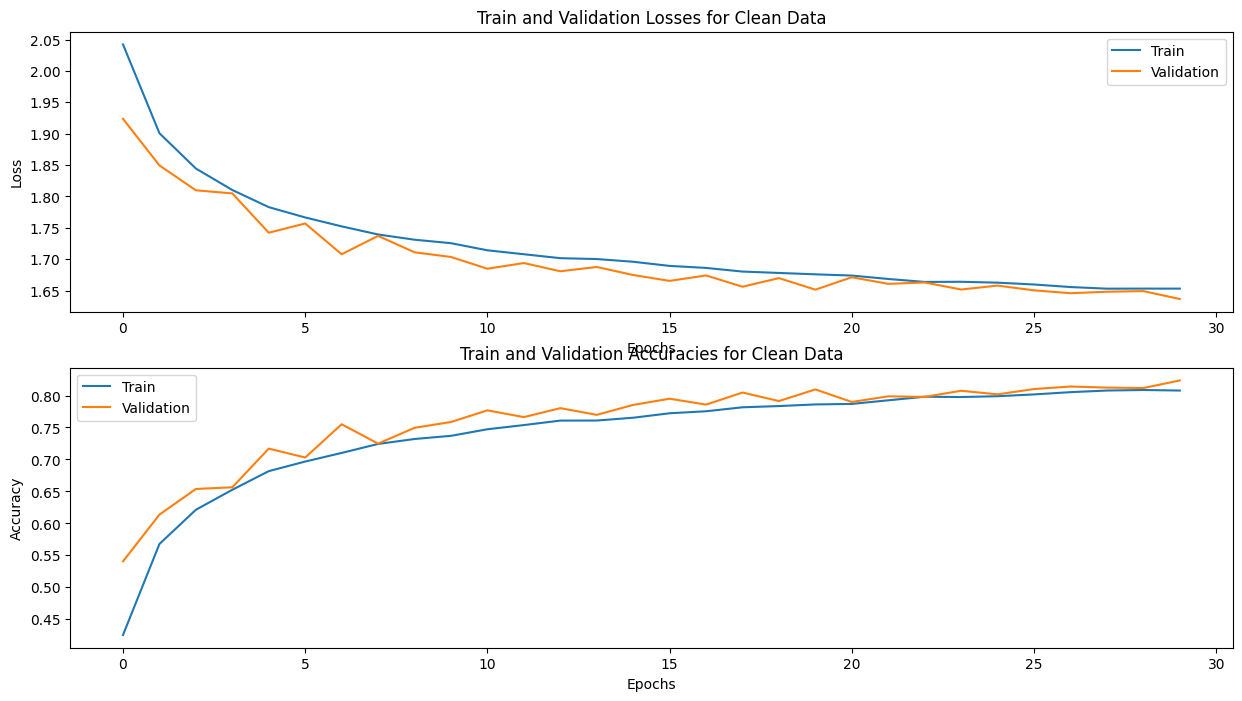
\includegraphics[width=1\textwidth]{curves_clean.png}
    \caption{Train and Test Accuracy and Loss curves for clean model.}
\end{figure}
\begin{figure}
    \centering
    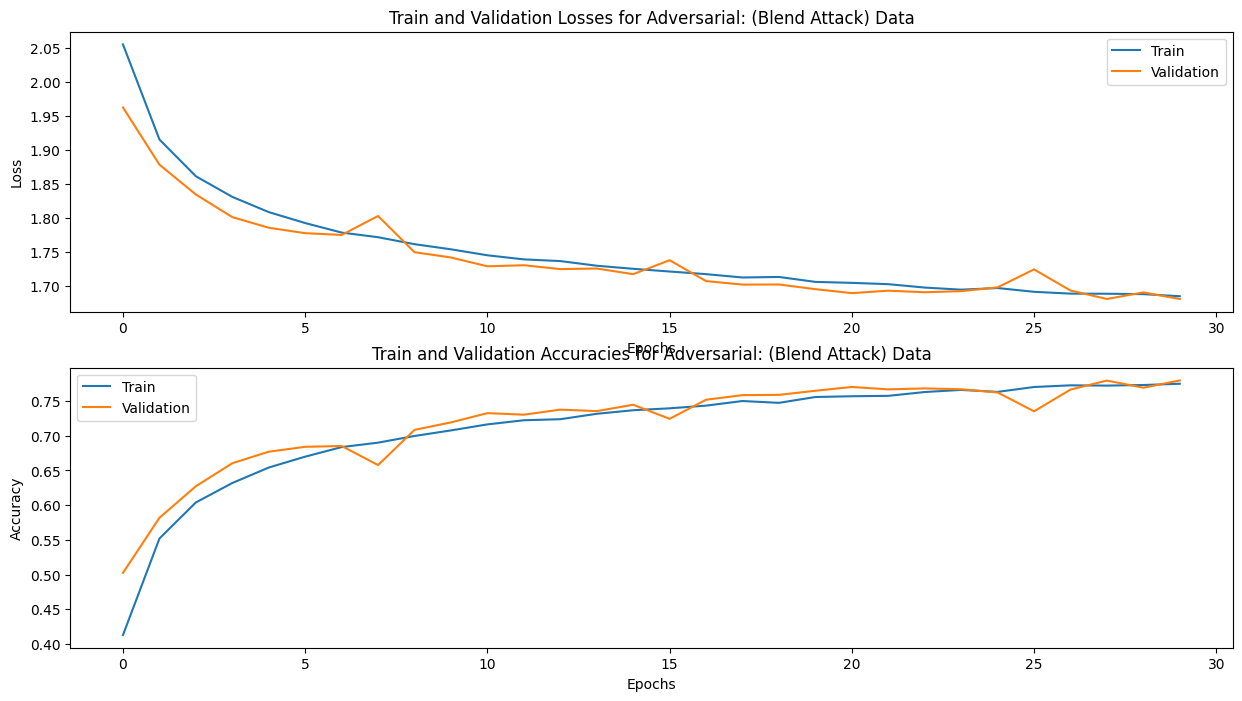
\includegraphics[width=1\textwidth]{curves_blend.png}
    \caption{Train and Test Accuracy and Loss curves for Blend-backdoored model.}
\end{figure}
\begin{figure}
    \centering
    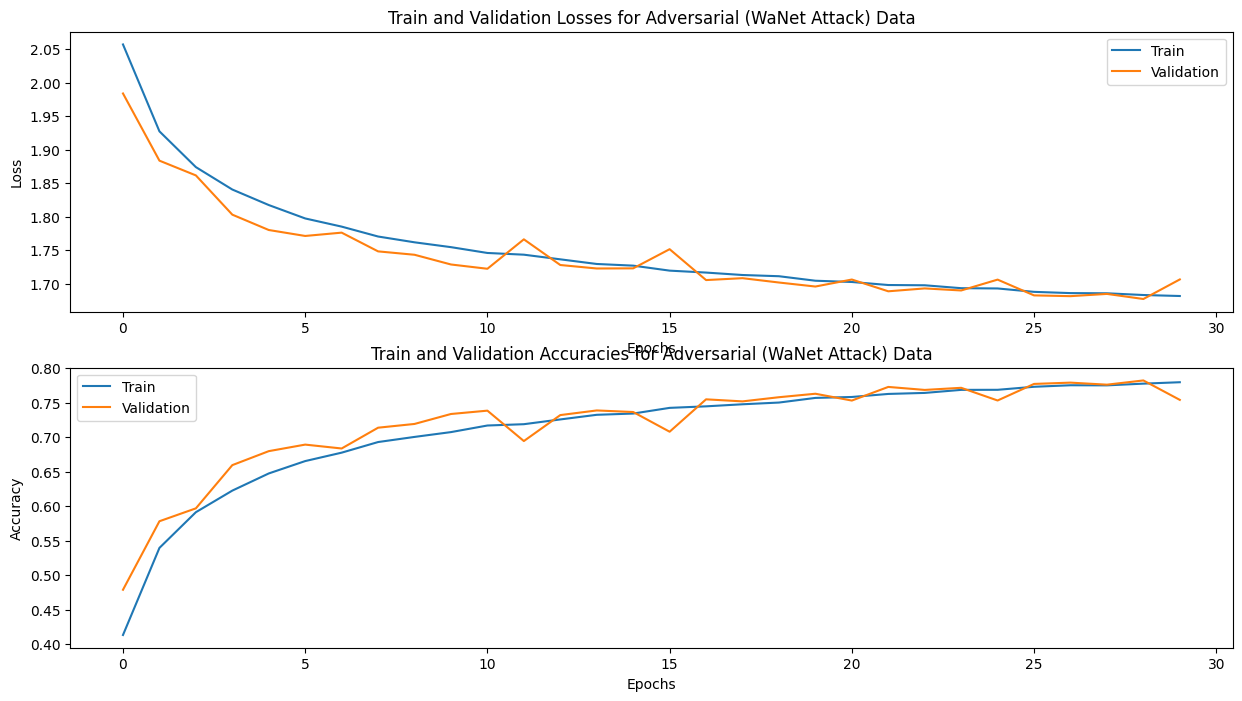
\includegraphics[width=1\textwidth]{curves_wanet.png}
    \caption{Train and Test Accuracy and Loss curves for WaNet-backdoored model.}
\end{figure}


\end{document}